
\section{Swap channels}

One of the major issues with direct ``on-chain'' payments in a blockchain network is that each transaction must be processed by each and every node participating in the network, resulting in high transaction costs.
One strategy to mitigate transaction costs is to defer payments and process them in bulk. In exchange for reduced cost, the beneficiary must be willing to incur higher risk of settlement failure.

\subsection{A simple chequebook}\label{subsec:simple-chequebook}

A very simple smart contract that allows the beneficiary to choose when payments are to be processed was introduced in \cite{ethersphere2016sw3}.
This \gloss{chequebook} contract is a wallet that can process cheques issued by its owner. The cheques are analogous to those in the real-world: the issuer signs a cheque specifying a beneficiary, a date and an amount, gives it to the recipient as a token of promise to pay at a later date. The smart contract plays the role of the bank. When the recipient wishes to get paid, they ``cash the cheque'' by submitting it to the smart contract. The contract, after validating the signature, date and the amount specified on the cheque, transfers the amount to the beneficiary's account (see figure \ref{fig:swap-chequebook}). Analogously to the person taking the cheque to the bank to cash it, anyone can send the digital cheque in a transaction to the owner's chequebook account and thus trigger the transfer. 

% Agents
\def\IssuerLocal{A client}
\def\IssuerSwapContract{A swap}
\def\BeneficiarySwapContract{B swap}
\def\BeneficiaryLocal{B client}

% Message Flows
\def\Issue{issue cheque}% \def\Cheque{Cheque}
\def\Redeem{redeem cheque} %\def\Cheque{Cheque}
\def\Clear{clear ETH} %\def\ETH{ETH}
\def\NW{withdrawal event} %\def\Msg{Log Event}
\def\ND{deposit event} %\def\Msg{Log Event}

% Legend 
\def\LegendOnChain{On-chain}
\def\LegendOffChain{Off-chain}

% Diagram
\begin{figure}
\centering
   
\begin{tikzpicture}[every node/.style={font=\small,
  minimum height=.35cm,minimum width=.5cm},]

%
% Matrix
\node [matrix, very thin,column sep=.6cm,row sep=0.2cm] (matrix) at (0,0) {
  & \node(0,0) (\IssuerLocal) {};   &                         & \node(0,0) (\IssuerSwapContract) {};   & & \node(0,0) (\BeneficiarySwapContract) {};   & & \node(0,0) (\BeneficiaryLocal) {}; \\
  & & & & & & & \\
  & & & & & & & \\
  & & & & & & & \\
  & \node(0,0) (\IssuerLocal 1) {}; & \node(0,0) (\Issue) {}; & \node(0,0) (\IssuerSwapContract 1) {}; & & \node(0,0) (\BeneficiarySwapContract 1) {}; & & \node(0,0) (\BeneficiaryLocal 1) {}; \\
  & & & & & & & \\
  & & & & & & & \\
  & \node(0,0) (\IssuerLocal 2) {}; &                         & \node(0,0) (\IssuerSwapContract 2) {}; & & \node(0,0) (\BeneficiarySwapContract 2) {}; & \node(0,0) (\Redeem) {};  &  \node(0,0) (\BeneficiaryLocal 2) {}; \\ 
  & & & & & & & \\
  & & & & & & & \\
  & \node(0,0) (\IssuerLocal 3) {}; &                         & \node(0,0) (\IssuerSwapContract 3) {}; & \node(0,0) (\Clear) {}; & \node(0,0) (\BeneficiarySwapContract 3) {}; &                    ; & \node(0,0) (\BeneficiaryLocal 3) {}; \\
  & & & & & & & \\
  & \node(0,0) (\IssuerLocal 4) {}; & \node(0,0) (\NW) {}   ; & \node(0,0) (\IssuerSwapContract 4) {}; &                         & \node(0,0) (\BeneficiarySwapContract 4) {}; & \node(0,0) (\ND) {}; & \node(0,0) (\BeneficiaryLocal 4) {}; \\
  & & & & & & & \\
  & \node(0,0) (\IssuerLocal 5) {}; &                         & \node(0,0) (\IssuerSwapContract 5) {};  & & \node(0,0) (\BeneficiarySwapContract 5) {};& & \node(0,0) (\BeneficiaryLocal 5) {}; \\
  & & & & & & & \\
  & \node(0,0) (\IssuerLocal 6) {}; &                         & \node(0,0) (\IssuerSwapContract 6) {};  & & \node(0,0) (\BeneficiarySwapContract 6) {};& & \node(0,0) (\BeneficiaryLocal 6) {}; \\
  & & & & & & & \\
  & \node(0,0) (\IssuerLocal 7) {}; & \node(0,0) (\LegendOnChain) {};  & & & & & \\
  & \node(0,0) (\IssuerLocal 8) {}; & \node(0,0) (\LegendOffChain) {}; & & & & & \\
};

% Agents labels
\fill 
	(\IssuerLocal) node[draw,fill=white] {\IssuerLocal}
	(\IssuerSwapContract) node[draw,fill=white] {\IssuerSwapContract}
	(\BeneficiarySwapContract) node[draw,fill=white] {\BeneficiarySwapContract}
	(\BeneficiaryLocal) node[draw,fill=white] {\BeneficiaryLocal};

\draw [dashed] 
  (\IssuerLocal) -- (\IssuerLocal 6)
  (\BeneficiaryLocal) -- (\BeneficiaryLocal 6)
  (\IssuerSwapContract) -- (\IssuerSwapContract 6)
  (\BeneficiarySwapContract) -- (\BeneficiarySwapContract 6);

% Horizontal flows (Monetary interactions)
%\draw [-latex] (\IssuerLocal 1) -- (\IssuerSwapContract 1.west) arc(180:0:0.37cm) -- (\BeneficiarySwapContract 1.west) arc(180:0:0.37cm) -- (\BeneficiaryLocal 1);
\draw [-{Latex[length=1.5mm,width=2.5mm]}] (\IssuerLocal 1) -- (\BeneficiaryLocal 1);
\draw [-{Latex[length=1.5mm,width=2.5mm]}] (\BeneficiaryLocal 2) -- (\IssuerSwapContract 2);
%\draw [-latex] (\BeneficiaryLocal 2) -- (\BeneficiarySwapContract 2.east) arc(0:180:0.37cm) -- (\IssuerSwapContract 2);
\draw [-{Latex[length=1.5mm,width=2.5mm]}] (\IssuerSwapContract 3) -- (\BeneficiarySwapContract 3);
\draw [-{Latex[length=1.5mm,width=2.5mm]}] (\IssuerSwapContract 3) -- (\IssuerLocal 4);
\draw [-{Latex[length=1.5mm,width=2.5mm]}] (\BeneficiarySwapContract 3) -- (\BeneficiaryLocal 5);

% Flows Labels 
\fill
  (\Issue) 
    node[above] {\Issue}
  (\Redeem) 
    node[above] {\Redeem}
  (\Clear) 
    node[above] {\Clear}
  (\NW) 
    node[above, text width=1.1cm,align=center,fill=white] {\NW}
  (\ND) 
    node[above, text width=1.5cm,align=center,fill=white] {\ND};

% Interaction points 
\draw 
  (\IssuerLocal 1) node[minimum size=0.25cm, draw,circle,fill=red!20] {}
  (\BeneficiaryLocal 1) node[minimum size=0.25cm, draw,circle,fill=red!20] {}
  (\BeneficiaryLocal 2) node[minimum size=0.25cm, draw,circle,fill=red!20] {}
  (\IssuerSwapContract 2) node[minimum size=0.25cm, draw,circle,fill=green!20] {}
  (\IssuerSwapContract 3) node[minimum size=0.25cm, draw,circle,fill=green!20] {}
  (\IssuerLocal 4) node[minimum size=0.25cm, draw,circle,fill=red!20] {}
  (\BeneficiarySwapContract 3) node[minimum size=0.25cm, draw,circle,fill=green!20] {}
  (\BeneficiaryLocal 5) node[minimum size=0.25cm, draw,circle,fill=red!20] {}
  (\IssuerLocal 7) node[minimum height=.1cm, minimum size=0.1cm, draw,circle,fill=green!20] {}
  (\IssuerLocal 8) node[minimum height=.1cm, minimum size=0.1cm, draw,circle,fill=red!20] {};

% Vertical lifelines
\draw [-{Latex[length=1.5mm,width=2mm]}] (\IssuerSwapContract 2) -- (\IssuerSwapContract 3);
 Legend labels
\draw
	(\LegendOnChain) node[minimum height=.1cm] {\LegendOnChain}
	(\LegendOffChain) node[minimum height=.1cm] {\LegendOffChain};
\end{tikzpicture}
\caption{The basic interaction sequence for swap chequebooks}
\label{fig:swap-chequebook}
\end{figure}

Since these digital cheques are files and can therefore be copied, care must be taken that the same cheque cannot be cashed twice. Such ``double cashing'' can be prevented by assigning each cheque given to a particular beneficiary a serial number which the contract will store when the cheque is cashed. The chequebook contract can then rely on the serial number to make sure cheques are cashed in sequential order, thus needing to store only a single serial number per beneficiary.
An alternative strategy to prevent double cashing, when repeated payments are made to the same beneficiary, is that the cheques contain the \emph{cumulative} total amount ever credited to the beneficiary. The total cumulative amount that has been cashed out is stored in the contract for each beneficiary. When a new cheque is submitted, the contract ignores cheques with amount equal to or less than the stored total, but it will transfer the difference if it receives a cheque with a higher total.

This simple trick also makes it possible to cash cheques in bulk because only the current `last cheque' need ever be processed. This achieves the reduction of transaction costs alluded to above.

Incidentally, the cumulative amount stored in the contract represents the total of all outgoing payments that have been honoured and thus the contract also serves as a credit history for the owner.

The amount deposited in the chequebook (\gloss{global balance}) serves as collateral for the cheques. It is pooled over the beneficiaries of all outstanding cheques.
In this simplest form, the chequebook has the same guarantee as real-world cheques: none. Since funds can be freely moved out of the chequebook wallet at any time, solvency at the time of cashing can never be guaranteed: if the chequebook's balance is less than the amount sanctioned by a cheque submitted to it, the cheque will bounce. This is the trade off between transaction costs and risk of settlement failure.


\subsection{SWAP accounting with chequebook}

Nonetheless, even in this simple form, the chequebook proves quite useful.
\cite{ethersphere2016sw3} introduces a protocol for peer to peer accounting, called \gloss{swap}.
\gloss{swap} is a tit-for-tat accounting scheme that scales microtransactions by
allowing service for service exchange between connected peers
(\emph{swap = swarm accounting protocol for service wanted and provided}).

In case of equal consumption with low variance over time, bidirectional services can be accounted for without any payments. Data relaying is such a service, making swap
ideally suited for implementing bandwidth incentives in content delivery or mesh networks.

\begin{center}
\begin{figure}
\begin{center}
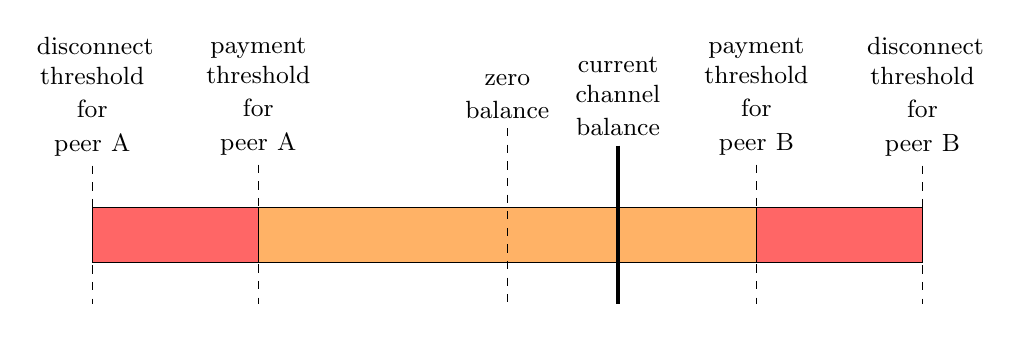
\begin{tikzpicture}
\node (middle)[draw, rectangle, fill=orange!60, minimum height=2em, minimum width=18em]{};
\node (leftred) [draw, rectangle, fill=red!60, minimum height=2em, minimum width=6em, node distance=12em,left of=middle]{};
\node (rightred)[draw, rectangle, fill=red!60, minimum height=2em, minimum width=6em, node distance=12em,right of=middle]{};
\node (zero) [above of=middle,node distance=5em, text width=4em, align=center] {\small zero\\ balance};
\node (zerod) [below of=middle] {};
\draw [dashed](zero)--(zerod);
\node (rtol) [node distance=9em,right of=zero,text width=4em, align=center] {\small payment\\threshold\\for peer B};
\node (rtold) [node distance=9em,right of=zerod] {};
\node (ltol) [node distance=9em,left of=zero,text width=4em, align=center] {\small payment\\threshold\\for peer A};
\node (ltold) [node distance=9em,left of=zerod] {};
\node (rdis) [node distance=15em, right of=zero,text width=4em, align=center] {\small disconnect\\threshold\\for peer B};
\node (rdisd) [node distance=15em,right of=zerod] {};
\node (ldis) [node distance=15em, left of=zero,text width=4em, align=center] {\small disconnect\\threshold\\for peer A};
\node (ldisd) [node distance=15em,left of=zerod] {};
\node (rbal) [node distance=4em,right of=zero,text width=4em, align=center] {\small current\\channel\\balance};
\node (rbald) [node distance=4em,right of=zerod] {};

\draw [dashed](rtol)--(rtold);
\draw [dashed](ltol)--(ltold);
\draw [dashed](rdis)--(rdisd);
\draw [dashed](ldis)--(ldisd);
\draw [very thick](rbal)--(rbald);
\end{tikzpicture}
\end{center}
\caption{Swap balance and swap thresholds.
Zero balance in the middle indicates consumption and provision are equal.
The current channel balance represents the difference in uncompensated service provision:
if to the right of zero, the balance tilts in favour of A with peer B being in debt, whereas to the left
the balance tilts in favour of B with A being in debt.
The orange interval represents loss tolerance. If the balance goes over the payment threshold, the party in
debt sends a cheque to its peer, if it reaches the disconnect threshold, the peer in debt is disconnected.}
\label{fig:swap}
\end{figure}
\end{center}


Extended with a delayed payment instrument like the chequebook, swap also offers a way to deal with unequal consumption
as well as high variance.
In the presence of high variance, or unequal consumption of services, the balance will eventually tilt significantly toward one peer. In this situation, the indebted
party issues a cheque to the creditor, to return the nominal balance to zero. This process is automatic and justifies swap as \emph{settle (the balance) with automated payments}
(see figure \ref{fig:swap}).

Such cheques can be cashed immediately by being sent to the issuer's chequebook contract. Alternatively, cheques can also be withheld
%. Withholding a cheque is effectively lending on credit, 
which enables the parties to save on transaction costs.
While, strictly speaking, there are no solvency guarantees, a bounced cheque will affect the issuer's reputation (as the chequebook contract records it).
On the premise that cheques are swapped in the context of repeating dealings, peers will refrain from
issuing cheques beyond their balance. In other words, interest in keeping good reputation with their peers is an incentive for maintaining solvency.

\begin{center}
\begin{figure}
\begin{center}
\begin{tabular}{ccc}
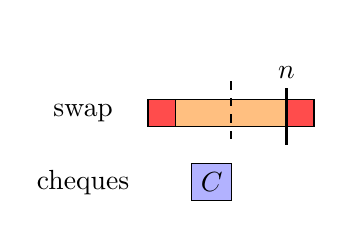
\begin{tikzpicture}
\node (middle)[draw, rectangle, fill=orange!50, minimum height=1em, minimum width=4em]{};
\node (leftred) [draw, rectangle, fill=red!70, minimum height=1em, minimum width=1em, node distance=2.5em, left of=middle]{};
\node (rightred)[draw, rectangle, fill=red!70, minimum height=1em, minimum width=1em, node distance=2.5em, right of=middle]{};
\node (zero) [above of=middle,node distance=2em, text height=1em] {};
\node (zerod) [below of=zero, node distance=3.5em] {};
\node (balance) [right of=zero,node distance=2em, text height=1.5em] {$n$};
\node (balanced) [below of=balance,node distance=3.5em] {};
\draw [dashed](zero)--(zerod);
\draw [very thick](balance)--(balanced);
\node (payment) [below of=zerod, node distance=1em]{};
\node (cheqeue) [draw, left of=payment, node distance=.7em, minimum height=1em, minimum width=1.4em, fill=blue!30, rectangle]{$C$};

\node (swap) [left of=leftred,minimum width=1em,align=right]{swap};
\node (cheques) [below of=swap,minimum width=1em, node distance= 2.5em, align=right]{cheques};
\end{tikzpicture}
&
\begin{tabular}{c}
  $\Longrightarrow$
\\ \\ \\ \\
\end{tabular}
&
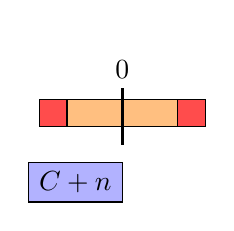
\begin{tikzpicture}
\node (middle)[draw, rectangle, fill=orange!50, minimum height=1em, minimum width=4em]{};
\node (leftred) [draw, rectangle, fill=red!70, minimum height=1em, minimum width=1em, node distance=2.5em, left of=middle]{};
\node (rightred)[draw, rectangle, fill=red!70, minimum height=1em, minimum width=1em, node distance=2.5em, right of=middle]{};
\node (zero) [above of=middle,node distance=2em, text height=1.5em] {$0$};
\node (zerod) [below of=zero, node distance=3.5em] {};
% \draw [dashed](zero)--(zerod);
\draw [very thick](zero)--(zerod);
\node (payment) [below of=zerod, node distance=1em]{};
\node (cheque) [draw, left of=payment, node distance=1.7em, minimum height=1em, minimum width=3.4em, fill=blue!30, rectangle]{$C+n$};
\end{tikzpicture}
\end{tabular}
\end{center}

\caption{Peer B's swap balance (with respect to A) reaches the payment threshold $n$ (left),
B sends a cheque to peer A. B keeps the cheque and restores the swap balance to zero.}
\label{fig:chequeswap}
\end{figure}
\end{center}

\subsection{Cancelling Cheques}

If the imbalance in the swap channel is the result of high variance as opposed to unequal consumption, after a period of accumulating cheques the channel balance starts tilting the other way. Normally it is now up to the other party to issue cheques to its peer resulting in uncashed cheques accumulating on both sides.
To allow for further savings in transaction costs, it could be desirable to be able to `play the cheques off against each other'.

Such a process is possible, but it requires certain deep changes within the chequebook contract. In particular, cashing cheques can no longer be immediate and must incur a security delay, familiar to anyone who has studied other implementations of payment channels.

Let us imagine a system analogous to cheques being returned to the issuer.  
Assume peer A issued cheques to B and the balance was brought back to zero. Later the balance tilts in A's favour but the cheques from A to B have not been cashed. In the real world, user B could simply return the last cheque back to A. In our case it is not so simple; we need some other mechanism by which B commits not to cash that particular cheque. Such a commitment could take many forms; it could be implemented by B signing a message allowing A to issue a new `last cheque` which has a lower cumulative total amount than before, or perhaps B can issue some kind of `negative` cheque for A's chequebook.

What all the implementations have in common, is that the chequebook can no longer allow instantaneous cashing of cheques. Upon receiving a cheque cashing request, the contract must wait to allow the other party in question to submit potentially missing information about cancelled cheques or reduced totals. 

We describe one possible implementation below.

\subsubsection{Waiving debt: bidirectional payments using a single chequebook }\label{subsubsec:waivingdebt}

To accommodate (semi-)bidirectional payments using a single chequebook we make the following modifications

\begin{enumerate}
    \item All cheques from user A to user B must contain a serial number.
    \item Each new cheque issued by A to B must increase the serial number.
    \item A's chequebook contract records the serial number of the last cheque that B cashed.
    \item During the cashing delay, valid cheques with higher serial number supersede any previously submitted cheques regardless of their face value.
    \item Any submitted cheque which decreases the payout of the previously submitted cheque is only valid if it is signed by the beneficiary.
\end{enumerate}

With these rules in place it is easy to see how cheque cancellation would work. 


Suppose user A has issued cheques $c_0 \ldots c_n$ with cumulative totals $t_0 \ldots t_n$ to user B. Suppose that the last cheque B cashed was $c_i$. The chequebook contract has recorded that B has received a payout of $t_i$ and that the last cheque cashed had serial number $i$.

Let us further suppose that the balance starts tilting in A's favour by some amount $x$. If B had already cashed cheque $c_n$, then B would now have to issue a cheque of her own using B's chequebook as the source and naming A as the beneficiary. However, since cheques $c_{i+1} \ldots c_n$  are uncashed, B can instead send to A a cheque with A's chequebook as the source, B as the beneficiary, with serial number $n+1$ and cumulative total $t_{n+1} = t_n - x$. Due to the rules enumerated above, A will accept this as equivalent to a payment of amount $x$ by B.

This process can be repeated multiple times until the cumulative total is brought back to $t_i$. At this point all outstanding debt has effectively been cancelled and any further payments must be made in the form of a proper cheque from B's chequebook to A.


\textbf{Suggestion - delete the rest of this subsection.}


In this scenario, instead of sending a cheque to A, B can waive part of their entitlement. This justifies swap as \emph{send waiver as payment} (see figure \ref{fig:waiverswap}).
A waiver essentially implements a proof that a cheque is destroyed and cannot be cashed, i.e., a promise that (part of) an uncashed cheque will not be redeemed.

A \gloss{waiver} is implemented as a note signed by the peer holding uncashed cheques %. The note specifies the current \gloss{swap index} (sequential number) 
 and indicates the amount of debt they agree to waive from their entitlement.

% \subsubsection*{Cashing cheques in the context of waivers}
If a channel is set to issue waived cheques then cashing must be a two step process.
Upon receiving a cheque, the contract verifies the data, and %signature and checks if the swap index matches the one on the cheque.
if the cheque is valid, the claimed amount is stored in a variable along with a timestamp. At this point a grace period starts: the original issuer gets notified of the cashing request and is invited to send in their last (highest) waiver signed by their peer. In case waivers are allowed cheques specify a \gloss{swap cycle index} and the contract keeps track of this.

% \subsubsection*{Cashing waivers}
Analogously to cheques, waivers are accepted by the contract. %if sent in as data in a transaction together with the issuer's address.
Upon receiving a waiver the contract verifies the data, and checks if the swap cycle index matches the one in the waiver.
If the waiver is valid, the peer's cumulative cashed balance is increased by the waived amount pretending the waived amount was paid out. Then the new cumulative cashed balance is compared to the one recorded when the cheque was received. Any remaining positive balance is transferred to the beneficiary, the cumulative sum is cleared from storage and the swap cycle index is incremented.

%%I stop here for now because the use of 'the swap index'  is confusing and I will rewrite it later ot be more clear.... a sequential index of waivers, stored by the checkbook separately from the serial number of the cheques but functioning like... how should this work? unclearly written

During the grace period the amount is not checked against the book's global balance.
After the grace period expires and no waiver was received, a second transaction
increments the swap cycle index and simply releases the funds or defaults on its debt.
During the grace period, further cheques can be sent to the contract: if they are valid and have the same swap cycle index as the one currently recorded, they simply replace the earlier one and the grace period is renewed.
Since waivers need to match the swap cycle index set by the cheques they destroy, they cannot be sent to the contract before the cheques they waive or after a new swap cycle starts.

In normal operation, however, peers are not incentivised to send in cheques as long as they can issue waivers. Once the waiver goes over the total amount of uncashed cheques, the peer needs to send a cheque. The swap cycle index is incremented in this cheque and the basis for issuing is the channel balance stored on the chain. This makes sure that cheques and waivers cannot be reused.%
%
\footnote{The volume of cheques waived will not increase the cumulative balance and therefore do not count toward total business volume for the purposes of credit history.
This can be amended if cheques are sent together with the latest waivers
and after validation the contract would adjust the cumulative balance to reflect the total volume.}

Using waivers can substantially increase the tolerated variance in the channel balance
without requiring actual transfer or impacting liquidity of the chequebook.
Without it, both peers would need to issue cheques and settlement would involve
transferring back and forth between the two peers, which means the first amount cashed
would not be available for a party for a period.

Waived cheques represent stronger guarantees since the cheque can effectively serve
as backing for incurring costs dedicated to the original issuer.

To summarise, Swap is ideally suited for immediately verifiable, recurring micropayments for bidirectional
services. The primary use case is bandwidth compensation and accounting to incentivise
relaying in a peer-to-peer system. As two peers are doing continuous business
they swap services, cheques and waivers and keep accounting and compensation offchain.




\begin{center}
\begin{figure}
\begin{center}
\begin{tabular}{ccc}
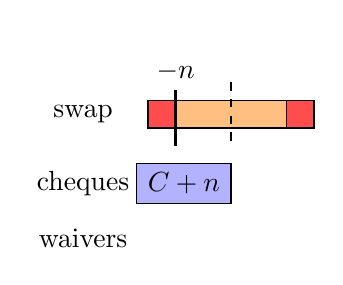
\begin{tikzpicture}
\node (middle)[draw, rectangle, fill=orange!50, minimum height=1em, minimum width=4em]{};
\node (leftred) [draw, rectangle, fill=red!70, minimum height=1em, minimum width=1em, node distance=2.5em, left of=middle]{};
\node (rightred)[draw, rectangle, fill=red!70, minimum height=1em, minimum width=1em, node distance=2.5em, right of=middle]{};
\node (zero) [above of=middle,node distance=2em, text height=1em] {};
\node (zerod) [below of=zero, node distance=3.5em] {};
\node (balance) [left of=zero,node distance=2em, text height=1.5em] {$-n$};
\node (balanced) [below of=balance,node distance=3.5em] {};
\draw [dashed](zero)--(zerod);
\draw [very thick](balance)--(balanced);
\node (payment) [below of=zerod, node distance=1em]{};
\node (cheque) [draw, left of=payment, node distance=1.7em, minimum height=1em, minimum width=3.4em, fill=blue!30, rectangle]{$C+n$};

\node (swap) [left of=leftred,minimum width=1em,align=right]{swap};
\node (cheques) [below of=swap,minimum width=1em, node distance= 2.5em, align=right]{cheques};
\node (waivers) [below of=cheques,minimum width=1em, node distance= 2em, align=right]{waivers};
\end{tikzpicture}
&
\begin{tabular}{c}
  $\Longrightarrow$
\\ \\ \\ \\
\end{tabular}
&
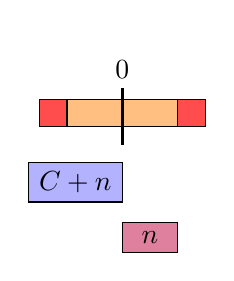
\begin{tikzpicture}
\node (middle)[draw, rectangle, fill=orange!50, minimum height=1em, minimum width=4em]{};
\node (leftred) [draw, rectangle, fill=red!70, minimum height=1em, minimum width=1em, node distance=2.5em, left of=middle]{};
\node (rightred)[draw, rectangle, fill=red!70, minimum height=1em, minimum width=1em, node distance=2.5em, right of=middle]{};
\node (zero) [above of=middle,node distance=2em, text height=1.5em] {$0$};
\node (zerod) [below of=zero, node distance=3.5em] {};
% \draw [dashed](zero)--(zerod);
\draw [very thick](zero)--(zerod);
\node (payment) [below of=zerod, node distance=1em]{};
\node (cheque) [draw, left of=payment, node distance=1.7em, minimum height=1em, minimum width=3.4em, fill=blue!30, rectangle]{$C+n$};
\node (waivers) [below of=payment, node distance=2em]{};
\node (waiver) [right of=waivers,minimum width=2em, node distance=1em,rectangle,draw,fill=purple!50]{$n$};
\end{tikzpicture}
\end{tabular}
\end{center}

\caption{Peer A's swap balance (with respect to B) reaches the payment threshold $n$ (left),
A sends a waiver to peer B. B keeps the waiver and restores the swap balance to zero}
\label{fig:waiverswap}
\end{figure}
\end{center}



\subsection{Channel deposits}

In what follows we extend the chequebook contract with the functionality of assigning per-user payout guarantees and show how two contracts having swap entries for each other constitute a full payment channel. 

\subsubsection{Payment channels}

A \gloss{payment channel} is a smart contract set up by two parties A and B and is used for secure bidirectional peer to peer payments off-chain. The contract has an amount of ether locked up in it that A and B have deposited. As the parties transact, they keep track of their \gloss{relative balance}, i.e., which portion of the locked up ether belongs to each party. The two parties A and B exchange signed messages agreeing on the current relative balance using some communication channel. If submitted to the channel contract, such messages change the balance. The messages sent back and forth function as payments between the two parties. Crucially, most of these messages are not submitted to the contract at all. The parties can choose to settle the new balance and record it in the channel contract by submitting the signed message in a transaction. The only time that balance has to be updated on-chain is when one party wishes to withdraw funds from the channel contract. Withdrawing funds requires a two step process.

A chequebook contract implementing a debt waiving procedure like the one outlined in section \ref{subsubsec:waivingdebt} shares a lot of the same features. If user A has deployed such a chequebook and is using it to pay user B, then the cheques act very similarly to the payment messages above, whereas the chequebook contract is analogous to a collection of half payment channels. Key differences to a full payment channel are 

\begin{enumerate}
    \item Payout is not guaranteed. 
    \item Initially payments can only flow in one direction (from A to B) 
    \item The balance can never go below zero i.e. in A's favour. This is why we refer to this construct as `half' of a payment channel. It is analogous to a payment channel in which the initial deposit was made only by A.
    \item Balances cannot be updated on-chain without a transfer. 
    \item All collateral locked to a node in the contract belongs to A; all that B can do is send in cheques to request a payout.% and then subsequently send the received funds to her own chequebook contract.
\end{enumerate}

In this section, we show how by adding channel deposits to the chequebook, it is possible to guarantee payouts to individual peers. When two chequebooks mutually have entry of each other, we can consider that as a full payment channel. We introduce a scheme that enables the chequebook owner to reallocate a global balance to individual peers in  a flexible way. Then we show how a strict protocol for shadowing outstanding liabilities can result in a novel enhanced full payment channel solution, called \gloss{swap channel}.

\subsubsection{Hard channel deposit}\label{subsubsec:per-user-guarantees}


Since cheques can bounce, payout is not guaranteed (see section \ref{subsec:simple-chequebook}). However, it is possible to add a payout guarantee to the cheques on a per-user basis. The chequebook deployed by user A has a balance of ether that acts as collateral for all outstanding cheques A has issued. We call this the \gloss{global balance}. As such, any user B holding a cheque from A has no guarantee that payout will be possible at any particular time in the future. 

To add a payout guarantee, we need to make some modifications to the contract. In order to be able to issue guaranteed cheques to user B, the contract would contain some ether that is locked in the contract and acts as collateral for payments from A to B only. Any cheques held by B are thus guaranteed to be honoured up to this locked amount, called \gloss{hard channel deposit}. In other words, the only way A can reclaim the locked amount is via a two step process that involves a payout request by A followed by a grace period during which B is still able to submit any outstanding cheques. With this mechanism in place, the chequebook is equivalent to a channel in which the entire initial deposit was made by A. 

If both A and B have such a chequebook contract, each having some collateral locked up for the other, then this setup is functionally equivalent to a full \gloss{payment channel}; with the exception that states can not be saved on the blockchain without an actual transfer. In existing payment channel proposals, the contract can update the \gloss{relative balance}, i.e., how much of the tied up collateral belongs to A and how much belongs to B. In the simple chequebook implementation such a re-balancing would involve a transfer from one chequebook contract to the other.%
%
\footnote{Advanced payment channels such as Raiden \cite{citation-needed:Raiden} have the ability to string together individual channels and compose them into a network. This extension is discussed in detail in section \ref{sec:networks}.}
%
The chequebook implementation has the advantage that it can start out simple with features being added gradually as they are needed.

The sum of all (hard) channel deposits is the \gloss{total channel deposit}. The global balance can never be less than the total of channel deposits. Channel deposit allocations can be controlled via transactions. Whenever a part of A's balance is assigned to B, the balance is checked and the transaction fails if total channel deposits would exceed the global balance.

Conversely, when the owner attempts to withdraw from the contract, the balance is not allowed to go below the total of channel deposits. 
The difference between the global balance and global deposit is the \gloss{liquid balance}. The total of channel deposits is never higher than the global deposit, the difference is \gloss{global liquid deposit} (see figure \ref{fig:balancesandeposits}).


\begin{center}
\begin{figure}
\begin{center}
\begin{tabular}{|c|c|c|c|c|c|c|c|c|c|}
\hline
\begin{tabular}{@{}c@{}}hard\\channel\\deposit\\ peer $p_0$\end{tabular} &
\begin{tabular}{@{}c@{}}hard\\channel\\deposit\\ peer $p_1$\end{tabular} &
...&
\begin{tabular}{@{}c@{}}hard\\channel\\deposit\\peer $p_n$\end{tabular} &
\begin{tabular}{@{}c@{}}soft\\channel\\deposit\\ peer $p_0$\end{tabular} &
\begin{tabular}{@{}c@{}}soft\\channel\\deposit\\ peer $p_1$\end{tabular} &
...&
\begin{tabular}{@{}c@{}}soft\\channel\\deposit\\ peer $p_n$\end{tabular} & 
{{\begin{tabular}{@{}c@{}}surplus\\ soft\\channel\\deposit\end{tabular}}}& 
{{\begin{tabular}{@{}c@{}}liquid\\ balance\end{tabular}}}
\\\cline{1-9}
\multicolumn{4}{|c|}{\begin{tabular}{@{}c@{}}total channel deposit\end{tabular}} &
\multicolumn{5}{|c|}{\begin{tabular}{@{}c@{}}global liquid deposit\end{tabular}} &
\\\cline{1-9}
\multicolumn{9}{|c|}{global deposit} & 
\\
\hline
\multicolumn{10}{|c|}{global balance}
\\
\hline
\end{tabular}
\caption{Chequebook balances and deposits.}
\label{fig:balancesandeposits}
\end{center}
\end{figure}
\end{center}



The question arises whether there is a way to distribute this global liquid deposit among the swap channels in a cost-effective, flexible yet secure way.%
%
\footnote{The global deposit can be implemented by the channel deposit assigned to the owner. Two step delayed withdrawal would fall out from this construct.}
%
At any point in time insolvency can be triggered if total uncashed balance is not covered by the global balance: $\sum_{i\in P}u_i > b$. On the other hand, solvency is guaranteed for peer B if the total of outstanding uncashed cheques from A to B is not greater than the total channel deposit ($u_B <= d_B$). If it is greater ($u_B > d_B$), part of A's liability is unsecured: $l_B = u_B - d_B$. If solvency is not guaranteed, it is reasonable for peer B to cash their cheque. If all peers do this, there is a bank run. If the sum of overruns is not greater than the liquid balance ($\sum_{i\in P}l_i <= l$, the bank run ends well, otherwise the creditors compete for liquidating their entitlement before the liquid balance runs dry. 
Insolvency is known if there is a peer whose unsecured uncashed balance is higher than the global liquid balance, i.e., $l_B > l$.
Solvency is not guaranteed if the unsecured balance is greater than zero. As the unsecured balance increases, so does the potential loss in case of insolvency. Is it possible to secure allocations of the liquid deposit so that it tracks the liabilities? 

\subsubsection{Soft channel deposit}

In the following we describe a construct which gives arbitrarily secure guarantee of solvency on the outstanding liabilities of peer A without explicitly assigning deposits to channels on chain.

Assume that there exist a notion of \gloss{epoch}, a fixed settlement period at the end of which B needs to sign off on the total sum of outstanding liability implied in the uncashed cheques issued by A to B.
Each time A sends a cheque to B they can offer to reallocate some of the surplus liquid deposit to B.
Formally, a \gloss{soft channel deposit note} is a signed note with the following fields:

\begin{itemize}
  \item creditor address
  \item debtor address
  \item the epoch index
  \item serial number
  \item channel balance
  \item soft channel allocation
\end{itemize}

If debtor signs it, the note is a \gloss{soft channel deposit offer}, if it is signed by the creditor and the note is \gloss{soft channel deposit claim}. As A is sending cheques to B, it can continually attach an increased soft channel deposit offer. As a response B accepts the offer by sending A a soft channel deposit claim of the offered amount (or less). Similarly, when B waives uncashed cheques from A, B attaches a (decreased) soft channel deposit claim to the waiver it is sending to A.

The soft channel deposit claim is the amount B would like to see secured/dedicated to them exclusively.
Assume that at the end of the epoch A's every  active peer has sent at least one claim to A.
After A receives soft channel deposit claims from all its active peers for the epoch, the claims are collected in a list (ordered according to the peer index of the beneficiary in A's swap contract). A signs the swarm hash of the (concatenated) list and sends it alongside the list to each peer
in a construct called a \gloss{soft channel deposit allocation table}.

Upon receiving the soft channel deposit allocation table, B verifies that
(1) the amount dedicated to B is no less than the total uncashed balance on matured cheques issued by A to B and
(2) the total sum of channel deposits allocated is no greater than the global deposit and
(3) each active peer in A's swap contract has a corresponding claim for the current epoch and 
(4) all the signatures are valid.
This process in illustrated in figure \ref{fig:softchanneldeposit}.
If soft channel offers and claims were issued according to the protocol, then (1) is automatically satisfied if A includes B's most recent claim. Points (2-4) make sure that each peer can make sure that the allocations are what the respective peers actually claim and their total does not exceed the global liquid deposit.

\begin{center}
\begin{figure}
\begin{center}
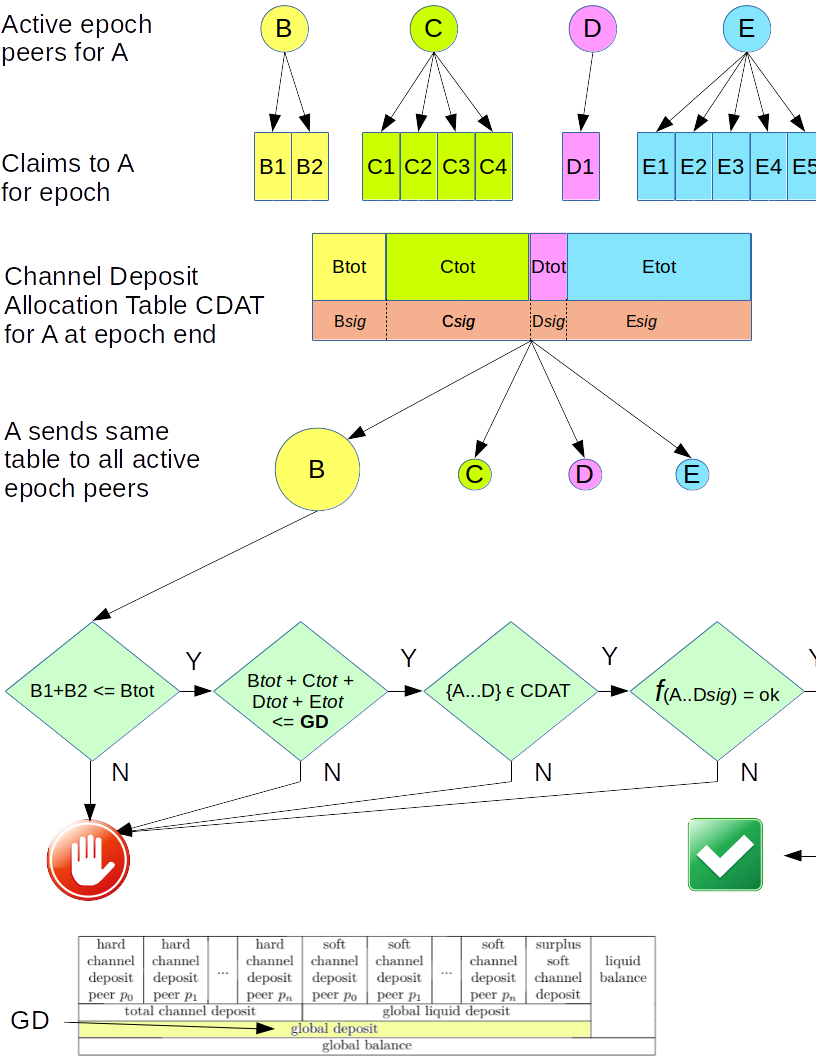
\includegraphics[scale=0.6]{diagrams/soft-channel.png}
%\begin{tikzpicture}
%\end{tikzpicture}
\end{center}
\caption{Hard and soft channel deposit}
\label{fig:softchanneldeposit}
\end{figure}
\end{center}


If the soft channel deposit allocation table is valid, B can with complete certainty know that the global deposit in A's contract has sufficient funds to cover all outstanding cheques handed to B even if all peers were to redeem all of their outstanding cheques and no further amount is deposited to increase the liquid deposit.
Practically, this means then that, after receiving a valid allocation table for the epoch from A, B has no risk of insolvency when holding out on cashing A's cheques. 

The hard channel deposit can serve as a secure buffer to allow increase in uncashed balance during the current epoch.
The sum of the currently allocated soft channel deposit and hard channel deposit is called channel deposit.
As long as the uncashed balance does not exceed the current channel deposit, solvency of A to B's claims is guaranteed. If the uncashed balance exceeds this limit, there is no guarantee that A will remain solvent, therefore B can just stop providing service. If the channel deposit  does not cover the uncashed balance, the result can be insolvency. If channel deposits cover the amount of uncashed cheques, the difference is called \gloss{surplus channel deposit}. As long as there is a surplus, A does not need to make an offer.

If we regard `accepting and not cashing cheques' as a service then we can define a higher level swap accounting. In a way, the hard channel deposit amount play the role of the payment  threshold in simple swap, whereas soft channel deposit offers and claims are somewhat analogous to cheques or waivers.
Instead of the dynamic swap cycle of the simple swap, here the cycle corresponds to an epoch. 

We can define a strict etiquette for the protocol. In the beginning, the allocated soft channel deposit from A to B is zero. As A sends a cheque to B in the amount of $x$ then it attaches an offer to raise the allocation from zero to $x$. Since the updates to the soft channel deposits only signalled after the epoch ends, accumulating cheques is risky if there is no guaranteed cover by per-user guarantee.
The hard channel deposit mitigates this by effectively backing up those outstanding notes that are issued during the current epoch. This effectively makes the hard channel deposit a throughput restriction on the channel traffic.  As a consequence, hard channel deposits are supposed to be chosen so that they reflect the desired per-epoch throughput of the channel.

This strict protocol has far-reaching consequences: (1) security, (2) instant payout and (3) unambiguous creditor. Firstly, A's peers cannot lose anything: Assume that B received additional cheques from A during the current epoch and accordingly issued claim to A to raise the soft channel deposit.  Imagine that the next soft channel allocation table is omitting A entirely or does not contain the most recent claim amount. However, since the increase is within the limit of the hard channel deposit, B can always enforce $100\%$ solvency.
Secondly, if we make the soft channel deposit claim contain the last serial number and swap balance, submitting the inclusion proof of the B's soft channel deposit claim in a valid current allocation table is sufficient to immediately release funds. 
Another important consequence of the strict protocol that at any one time only one of two connected peers is sending an allocation table to the other. The recipient can use the received one as evidence that the peer claim is zero and include it in their allocation table. 

\subsubsection{Unique allocation and double spending}

So far we just assumed that all peers can give a valid claim at the end of the epoch. 
If there is no absolute consensus on who participates, peers could be given alternative allocations by A. Two groups of nodes would be made to believe they are the unique descendent of the original group (e.g., the entire set of all peers that has an entry in A's contract). The allocation table signs off on the active participants.
If we simply allow the active peer set to change from one epoch to the next, a malicious node can start issuing alternative allocation tables to two sets of peers. Naive nodes in either set would think their set represents the entire active set. Colluding adversaries in both groups would sign off on reduced allocations which then can be used to cover the increased allocations of victims in both groups. The victims incorrectly assume the allocation table is exhaustive, i.e., it contains all peers whose allocation can increase: as long as they will accept their allocation table valid, they can be exploited with such a continuous double spend attack until they decide to settle on the blockchain. To mitigate this attack, one has to make sure that the active peer set does not split. Even though it would be possible for peers to agree on the allocation in a multiparty state channel with unanimous consensus rule, this suffers from the same availability issue as the one it is trying to solve.

Adding new peers to the allocation table is always possible, so is increasing the channel deposits unilaterally. However, dropping peers from a table can be problematic unless we are certain that A does not allocate multiple tables to victims.
We propose instead that it is A's responsibility to prove off-chain that they issue a unique allocation table. 
If we can make sure that A issues a unique resource update for the active set in every epoch, then changing peer set is no longer a problem. 
Assume that C formerly included in the allocation table is presented with a new table with some earlier peers missing, then they must verify somehow that the table is unique. 

A protocol called \gloss{mutable resource update notifications} offers a solution: 
The pull notification version requires the resource owner to send a \gloss{resource update chunk} to a number of deterministic but not predictable addresses. These are stored and served exactly as chunks, except that their validity is not verified by checking  their address against the swarm hash of their content but the signatures against its uniqueness. Now assume a malicious node A and its colluding peers achieve a situation when they sign on alternative allocation tables to two groups each containing a naive node B and C, respectively. When B and C are in their respective split, then both B and C check A's resource updates at the same time. In order for A to keep up a double spend attack against B and C then B and C must receive the two allocation tables as a result to their query of the resource update chunk. In other words, adversary A needs to make sure each of the two versions is served to the respective peer that expects it. 
But this is not easy. With nodes incentivised to report multiple signing, the adversary would have to (1) be able to identify which incoming request originates from B and C%
%
\footnote{Due to sender anonymity in retrieval, requests cannot easily be linked to the originators' identity, although direction where the request is coming from can be. The scheme can be strengthened by requiring entire neighbourhoods to sign off on the uniqueness and increase the stake., i.e. if they are caught giving out different updates under the same address, they can be challenged on the blockchain and lose their deposit. See section \ref{sec:courtroom} for how such promises can be guaranteed. Alternatively, multiple addresses for a single update could be required.
As the number of required addresses (neighbourhoods) for a single update increases, the probability of uniqueness multiplies, essentially to allow arbitrary level of certainty.}
%
and (2) bribe all nodes involved in the retrieval to collude.
This uses the power of the big network to make it impossible for adversaries to fork on the truth.
%https://gist.github.com/zelig/895563df3357ef862f30be5c4344e63f

In summary, using soft channel deposits enables the chequebook owner to allocate and reallocate funds from their liquid deposit as channel deposits each dedicated to one particular peer. 
This construct offers a way for A's peers to hold out on cashing beyond the hard channel deposit. As long as the overall debt across channels remains below the global channel deposit this  allows us to overcome high variance in debt across epochs and peers in a fairly flexible way without blockchain transaction costs, yet provides very strong guarantees there is a consensus among A's peer with regards to the allocation. 

\subsection{Zero cost entry}

Swap accounting can also work in one direction only. If a party enters the system with zero ether (\gloss{newcomer}), but connects to peers with funds (\gloss{insider}), the newcomer begins to provide the service (and not use it) in order to earn a positive swap balance. Once the payment threshold is reached, the newcomer will be paid and is soon able to deploy chequebook of her own.
In short, even without any chequebook contract at all, Swap offers zero cost onboarding to newcomers. Once the payout threshold is reached, the insiders could pay the newcomers on-chain. 

If the insider has a chequebook and wishes to pay the newcomer with a cheque, this is also possible, but there is a caveat here in that cashing cheques requires sending a transaction to the blockchain, and therefore: gas.%
%
\footnote{Although this restriction may be dropped once ethereum is upgraded to the `Metropolis' release in which the chequebook contract will be able to pay for the transfer and deduct the cost of the transfer from the payout.}
%
The newcomer will be able to earn cheques for services provided, but will not have the means to cash them. 
Unless the first payment is an on-chain payment or the node can convince one of its peers to send the transaction for them.


We allow nodes to sign off on a structure, and extend the swap contract with a preprocessing step, which triggers payment to the transaction sender covering the transaction's gas cost plus a service fee.

  
  
A newcomer connects to  an insider with an existing chequebook contract. The insider consumes the newcomer's services and instead of issuing a cheque, the insider agrees to create a chequebook contract for the newcomer. When the insider's service debt reaches the amount needed for contract creation, the insider sends a transaction to create the contract with newcomer as the owner. Once the newcomer has her own chequebook contract, she is able to consume services and issue cheques to pay for them.
 
In order to be useful however, the deployed chequebook must also have some positive balance as collateral. Since the newcomer has no ether, it must be the insiders who deposit this starting balance. If peers agreed that they want to save on transaction costs, it is reasonable to create the contract with the required initial balance in one go. This would imply waiting out with contract creation until the insider's debt reaches the \emph{cost of bootstrapping} which is the sum of (1) the cost of contract creation, (2) the required starting balance, and (3) possibly some extra service fee to incentivise insiders to provide this kind of service.

\begin{center}
\begin{figure}
\begin{center}
\end{center}
\caption{Bootstrapping or how to launch as a swap capable node consuming and providing a
service  and earn money}
\label{fig:bootstrapping}
\end{figure}
\end{center}


To summarise, by serving before consuming, participants can bootstrap their way into swap without the need for funds. Hence swap is justified as (\emph{setting up a wallet as payment}).
